\section{Wyniki testów}

\begin{frame}
	\frametitle{Scenariusz testu funkcjonalnego}
	\begin{block}{Założenia testu}
		W ramach testu funkcjonalnego, wykonane zostanie test polegający na:
		\begin{itemize}
			\item podjechaniu do szafki,
			\item otworzeniu szafki,
			\item wyciągnięciu przedmiotu z szafki,
			\item podjechaniu do stołu,
			\item odłożeniu przedmiotu na stół.
		\end{itemize}
	\end{block}
\end{frame}

\begin{frame}
	\frametitle{Szczegóły implementacyjne}
	Przed wykonaniem testu zdecydowano się na kilka założeń upraszcających:
	\begin{itemize}
		\item pozycja obiektów jest znana,
		\item wykorzystana jest wcześniej przygotowana mapa statyczna,
		\item pomiędzy punktami docelowymi nie ma nieznanych przeszkód.
	\end{itemize}
\end{frame}

\begin{frame}
	\frametitle{Świat symulacji}
	\begin{figure}[b]
        \label{sim_world}
        \centering
        \def\svgwidth{\columnwidth}
        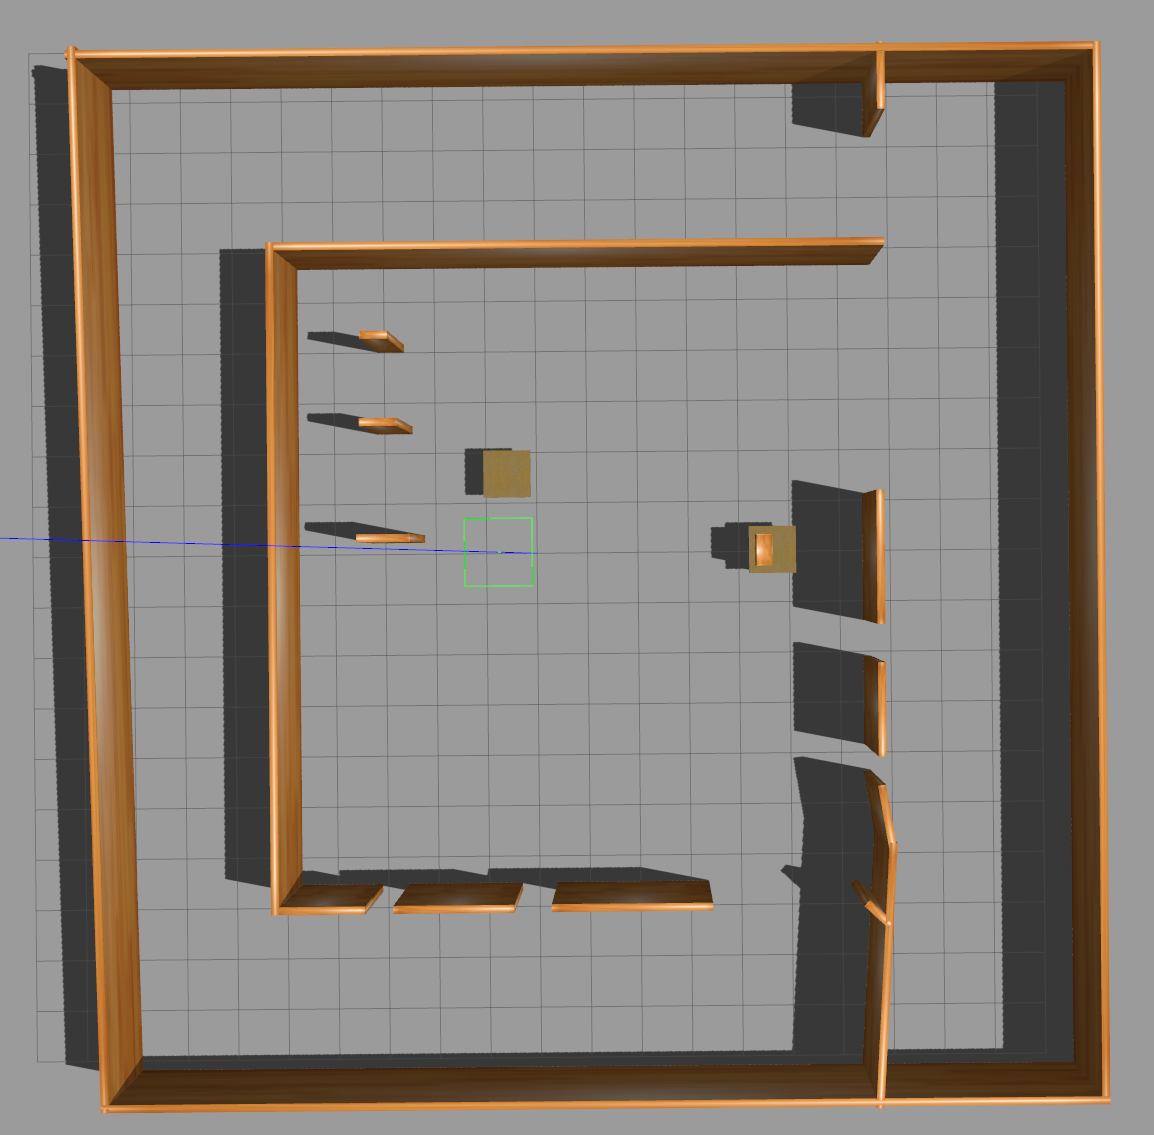
\includegraphics[scale=0.23]{images/gazebo_world.png}
        \caption{Świat symulacji w Gazebo}
    \end{figure}
\end{frame}

\addtocounter{framenumber}{-1}
\begin{frame}
	\frametitle{Świat symulacji}
	\begin{figure}[b]
        \label{sim_map}
        \centering
        \def\svgwidth{\columnwidth}
        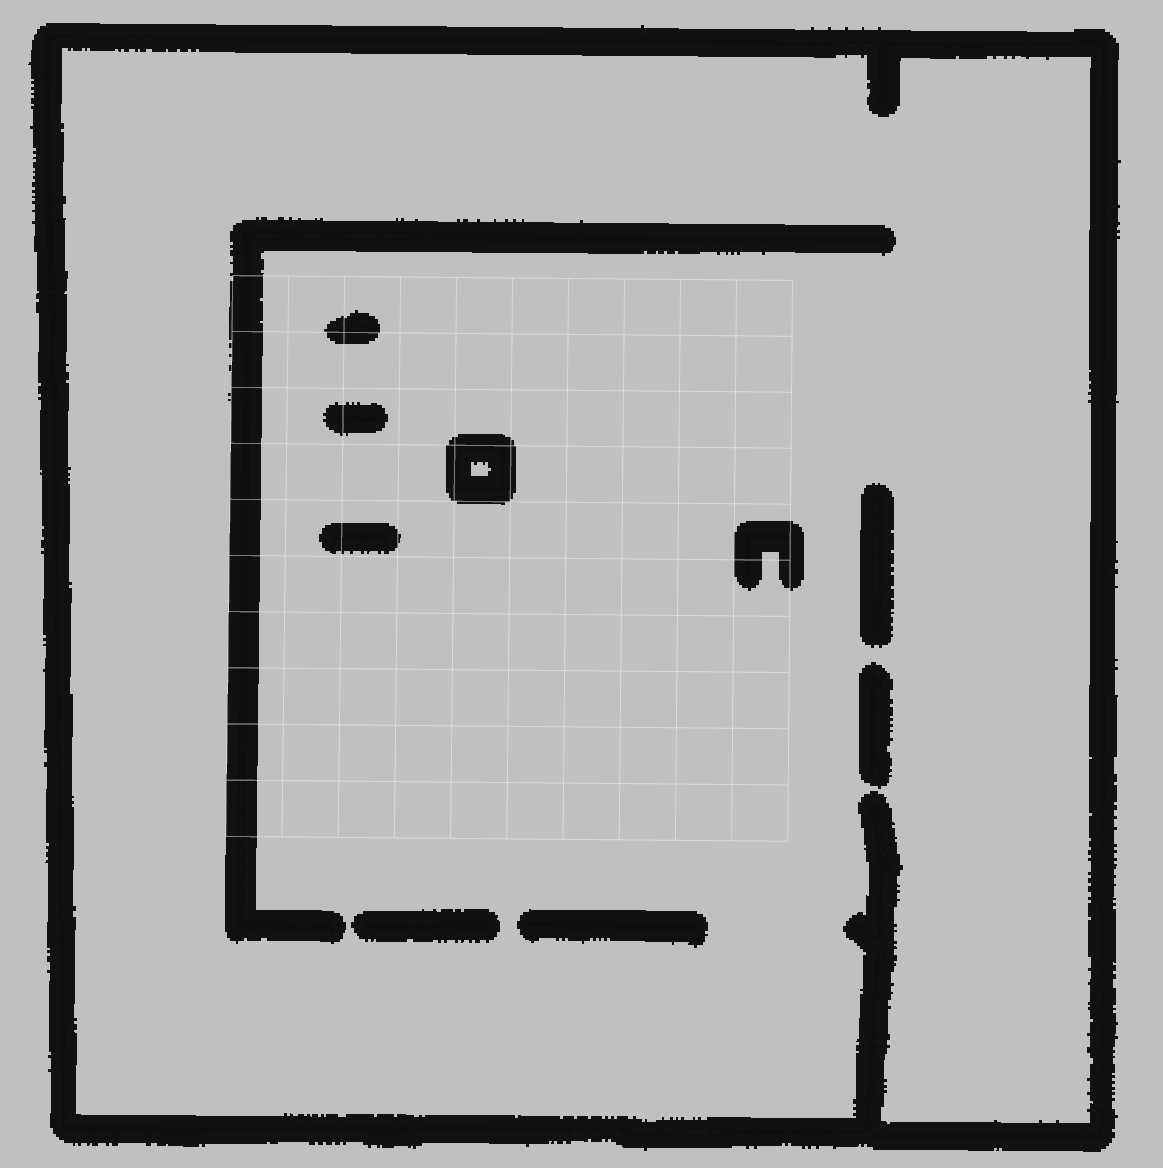
\includegraphics[scale=0.22]{images/static_map.jpg}
        \caption{Odpowiadająca światowi symulacji, statyczna mapa otoczenia w Rviz}
    \end{figure}
\end{frame}

\begin{frame}
	\frametitle{Realizacja testu}
	\begin{figure}[b]
        \label{sim_map}
        \centering
        \def\svgwidth{\columnwidth}
        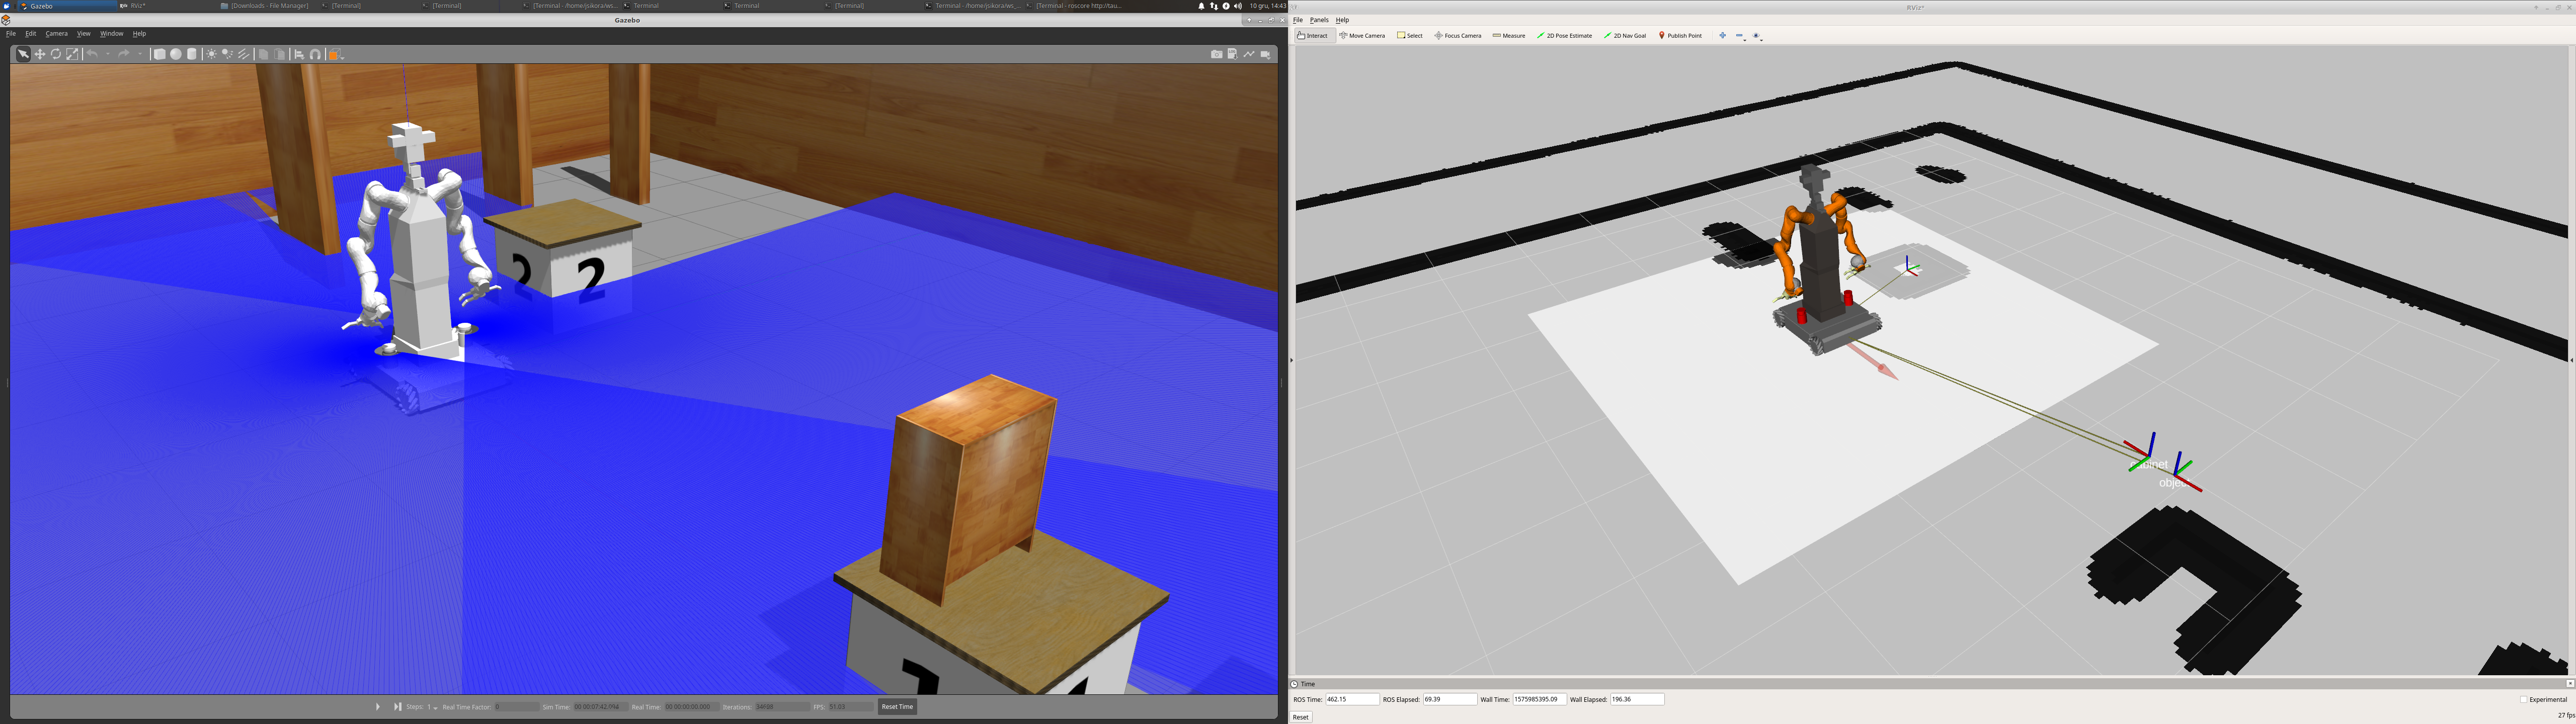
\includegraphics[scale=0.25]{images/testpuszka/start.png}
        \caption{Pozycja startowa}
    \end{figure}
\end{frame}

\addtocounter{framenumber}{-1}
\begin{frame}
	\frametitle{Otwieranie szafki}
	\begin{figure}[b]
        \label{sim_map}
        \centering
        \def\svgwidth{\columnwidth}
        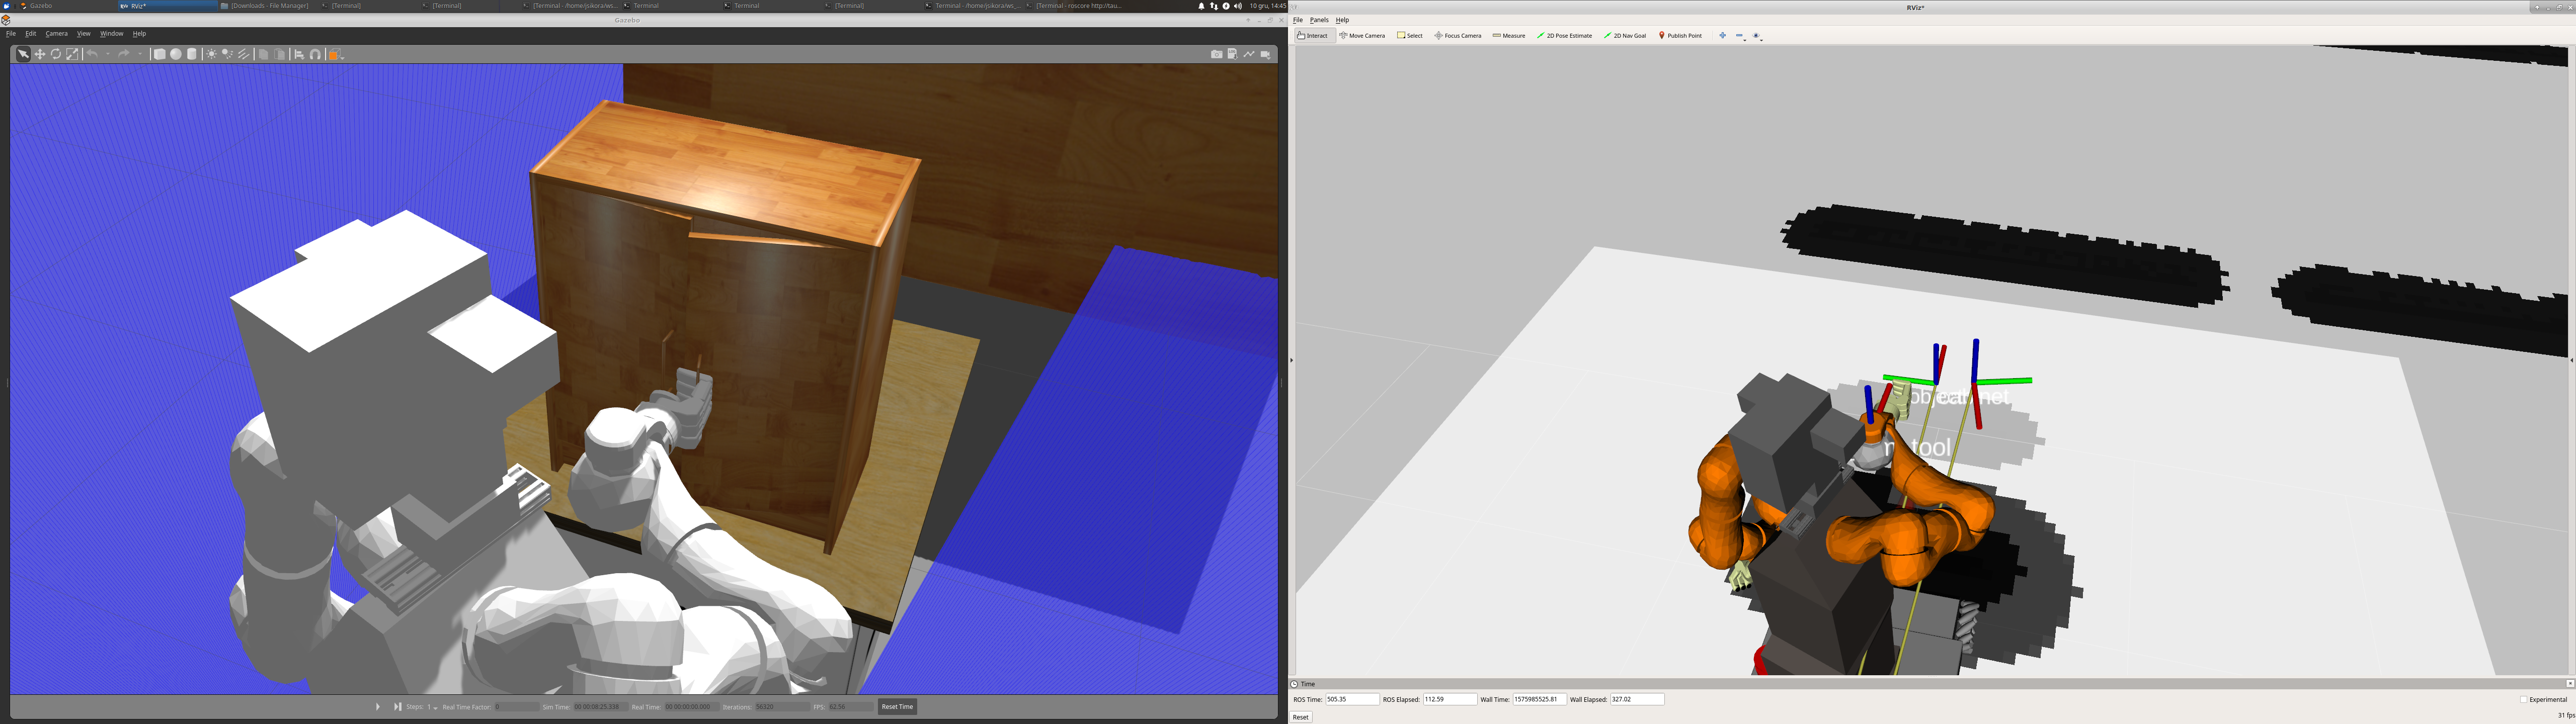
\includegraphics[scale=0.25]{images/testpuszka/otwieranie_start.png}
        \caption{Otwieranie szafki, krok 1}
    \end{figure}
\end{frame}

\addtocounter{framenumber}{-1}
\begin{frame}
	\frametitle{Otwieranie szafki}
	\begin{figure}[b]
        \label{sim_map}
        \centering
        \def\svgwidth{\columnwidth}
        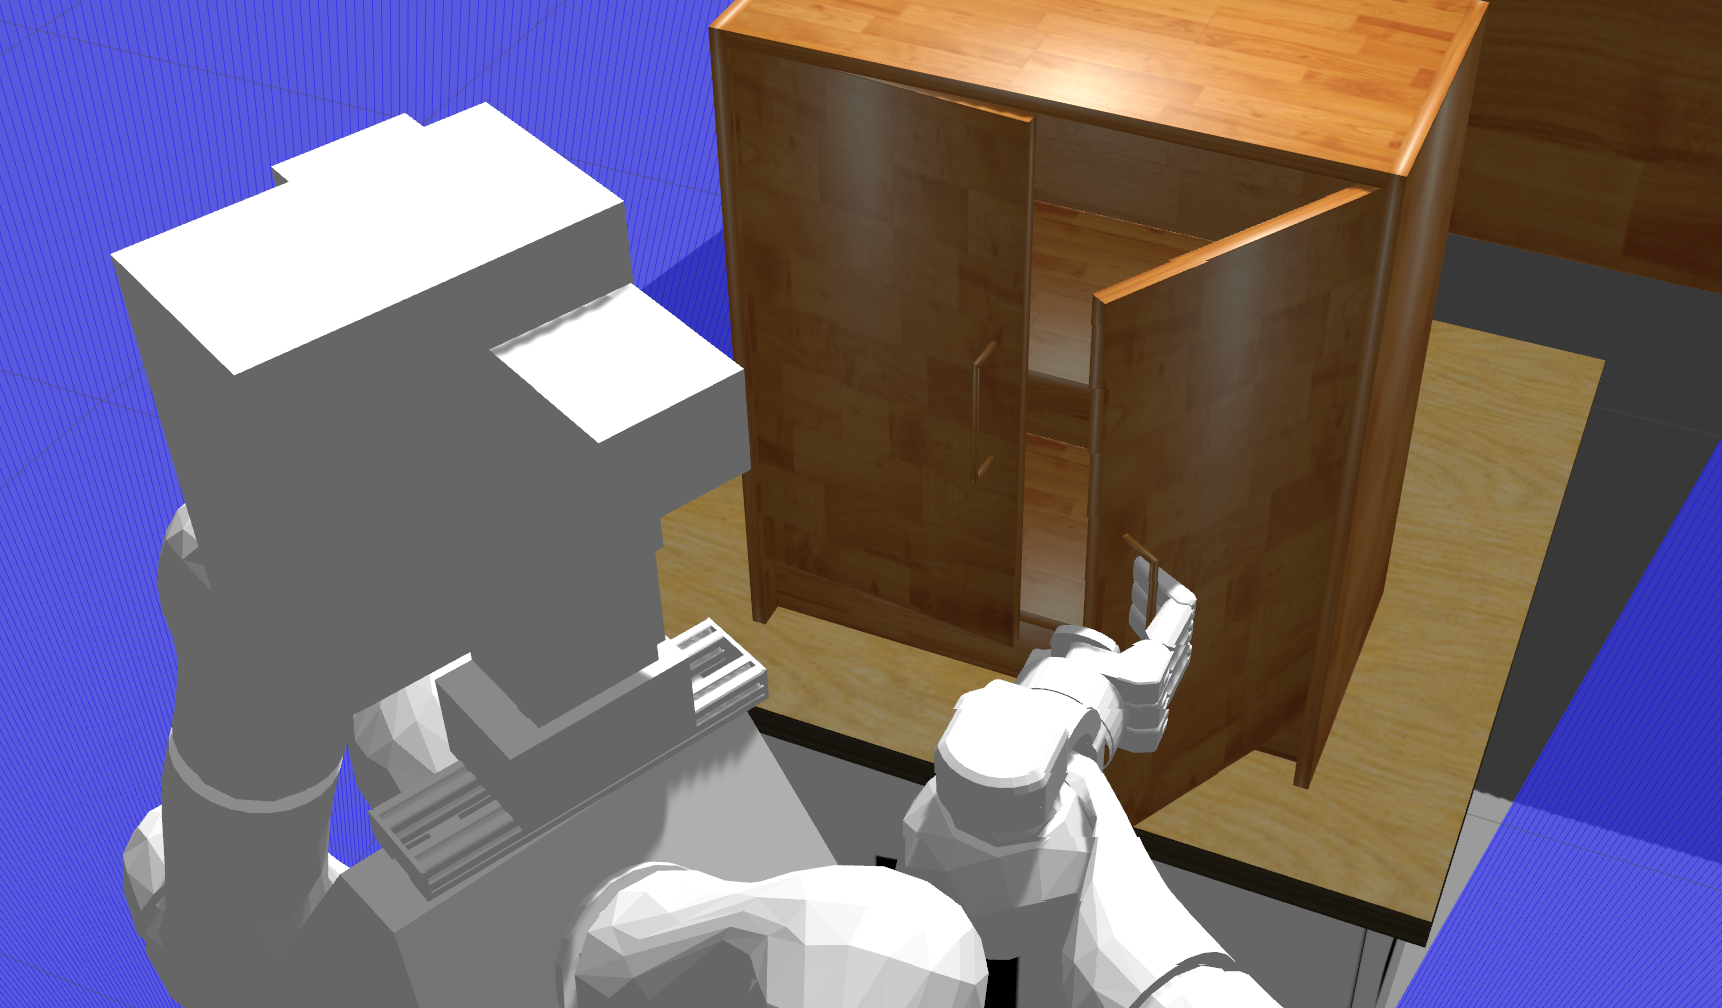
\includegraphics[scale=0.25]{images/testpuszka/otwieranie_koniec.png}
        \caption{Otwieranie szafki, krok 2}
    \end{figure}
\end{frame}

\addtocounter{framenumber}{-1}
\begin{frame}
	\frametitle{Otwieranie szafki}
	\begin{figure}[b]
        \label{sim_map}
        \centering
        \def\svgwidth{\columnwidth}
        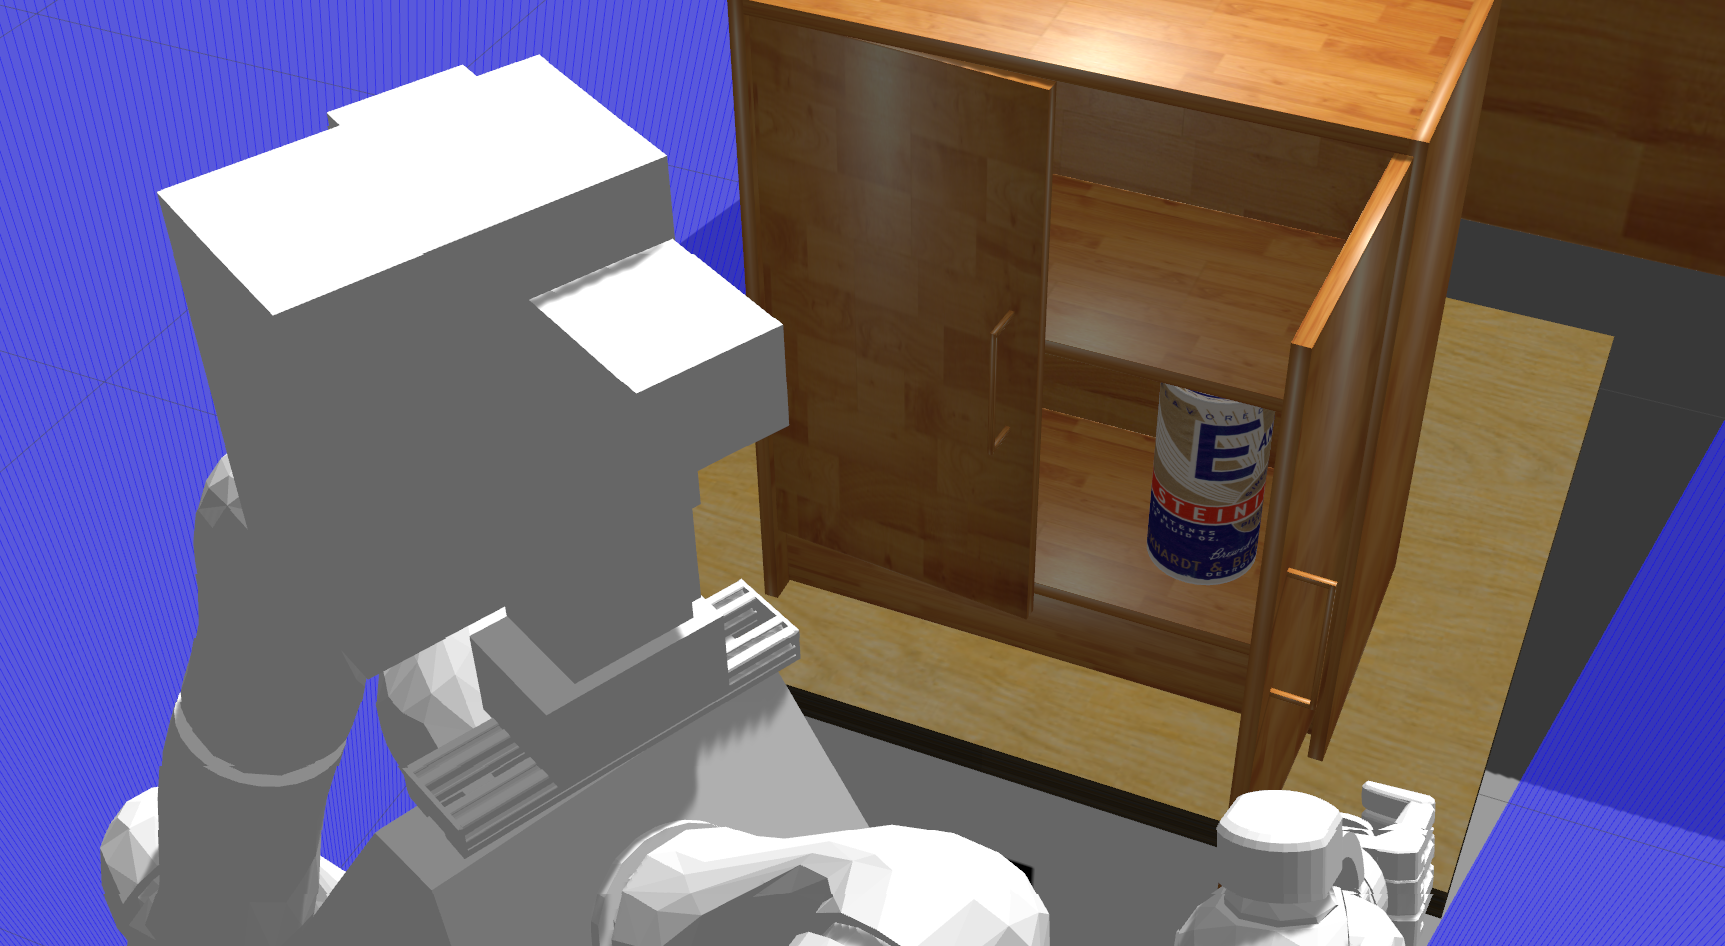
\includegraphics[scale=0.25]{images/testpuszka/otwarta_szafka.png}
        \caption{Otwieranie szafki, krok 3}
    \end{figure}
\end{frame}


\begin{frame}
	\frametitle{Wyciąganie puszki}
	\begin{figure}[b]
        \label{sim_map}
        \centering
        \def\svgwidth{\columnwidth}
        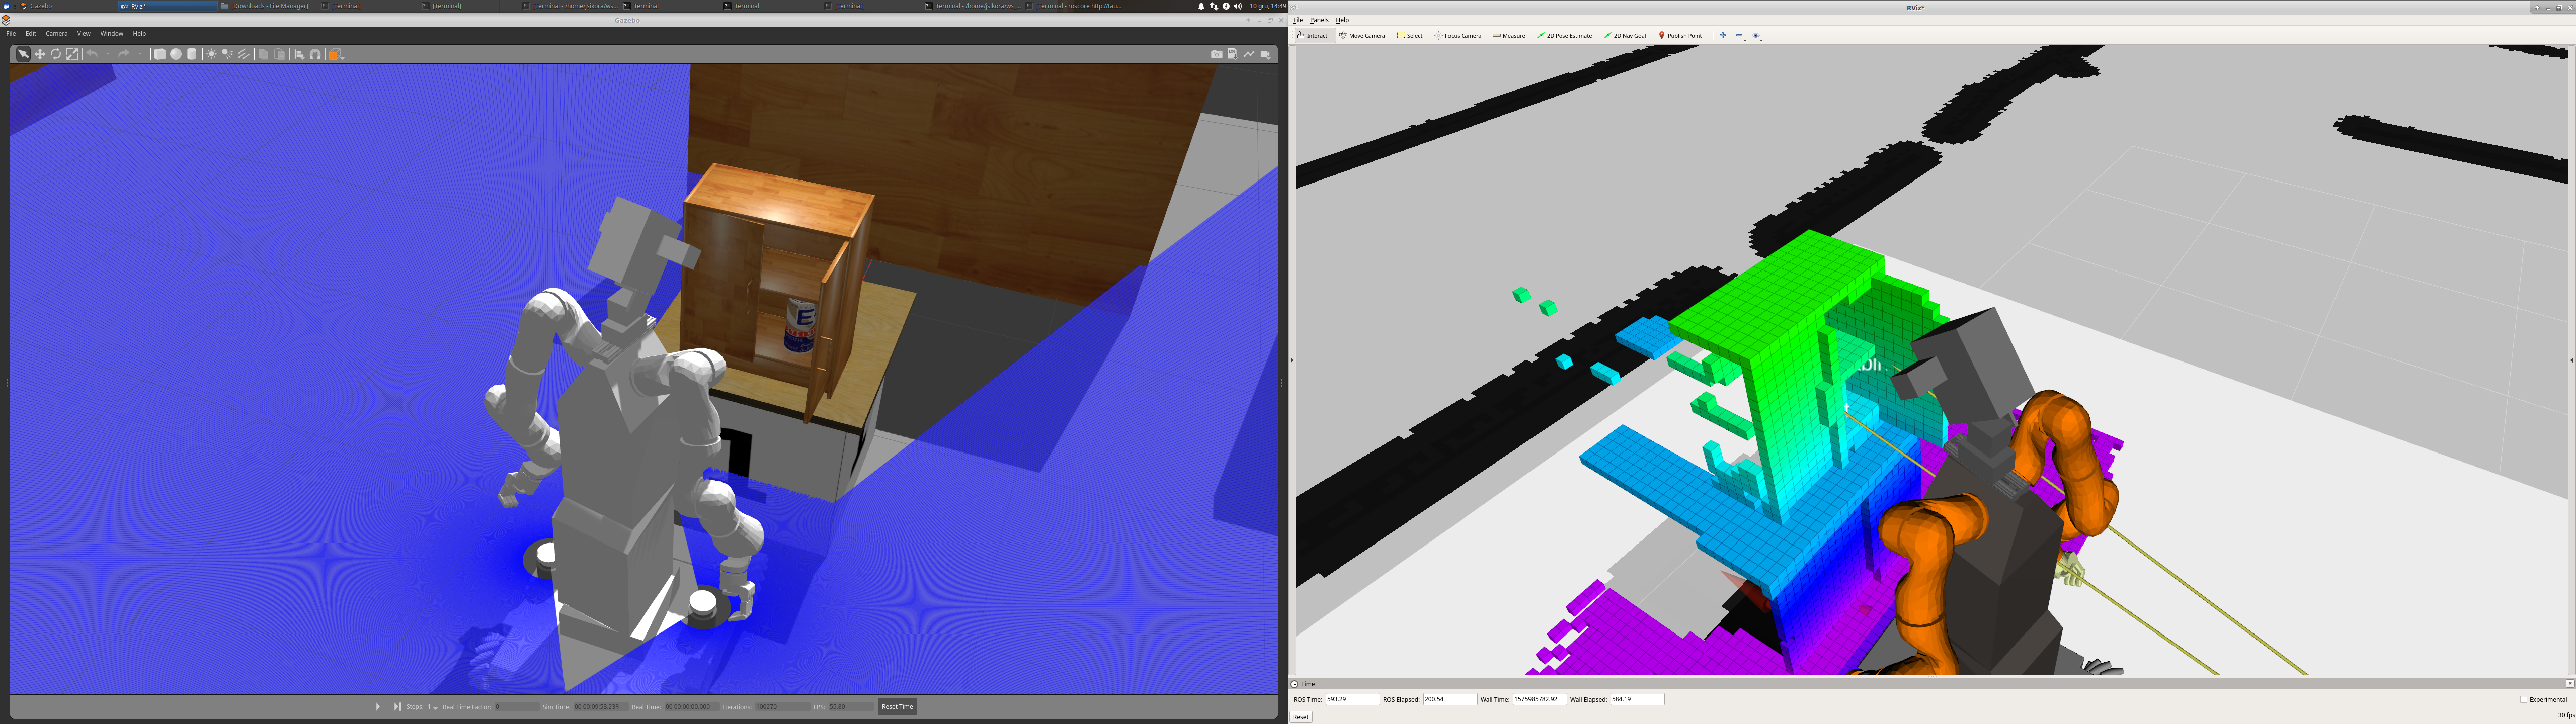
\includegraphics[scale=0.33]{images/testpuszka/wykrywanie_octomapy.png}
        \caption{Aktualizacja mapy otoczenia}
    \end{figure}
\end{frame}

\addtocounter{framenumber}{-1}
\begin{frame}
	\frametitle{Wyciąganie puszki}
	\begin{figure}[b]
        \label{sim_map}
        \centering
        \def\svgwidth{\columnwidth}
        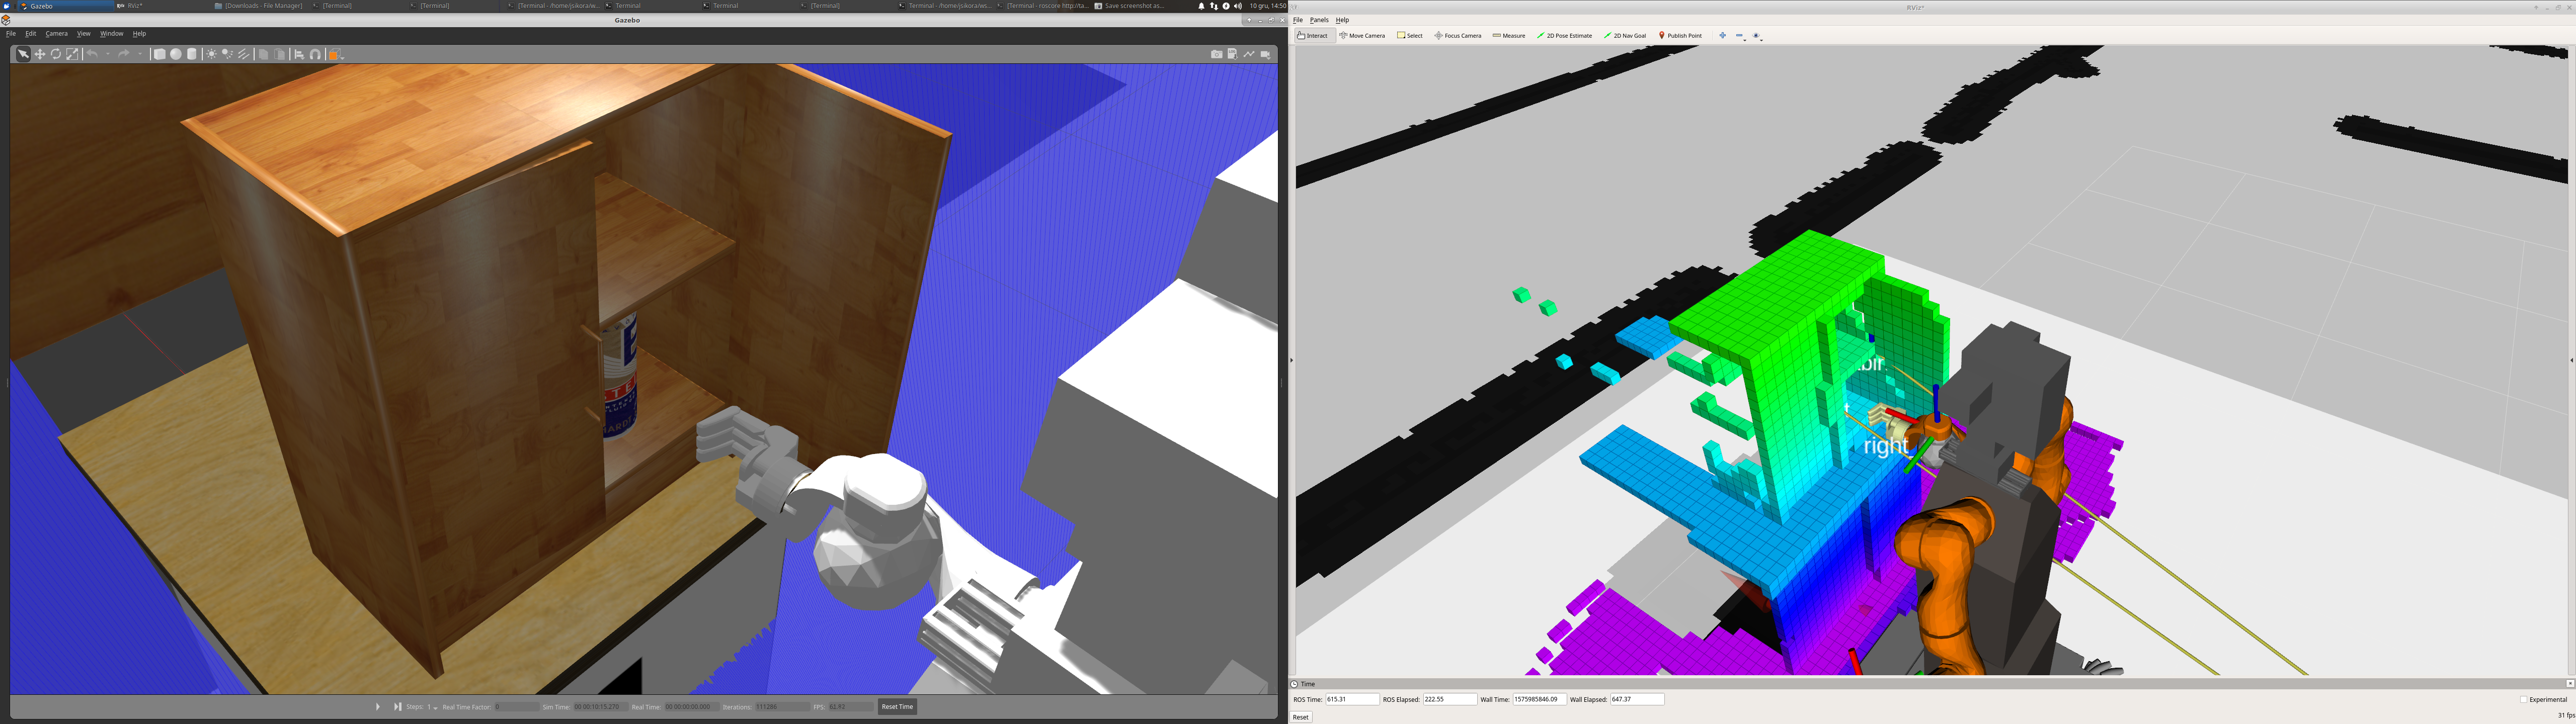
\includegraphics[scale=0.3]{images/testpuszka/najazd_reka_na_psuzke.png}
        \caption{Najazd ręką na obiekt}
    \end{figure}
\end{frame}

\addtocounter{framenumber}{-1}
\begin{frame}
	\frametitle{Wyciąganie puszki}
	\begin{figure}[b]
        \label{sim_map}
        \centering
        \def\svgwidth{\columnwidth}
        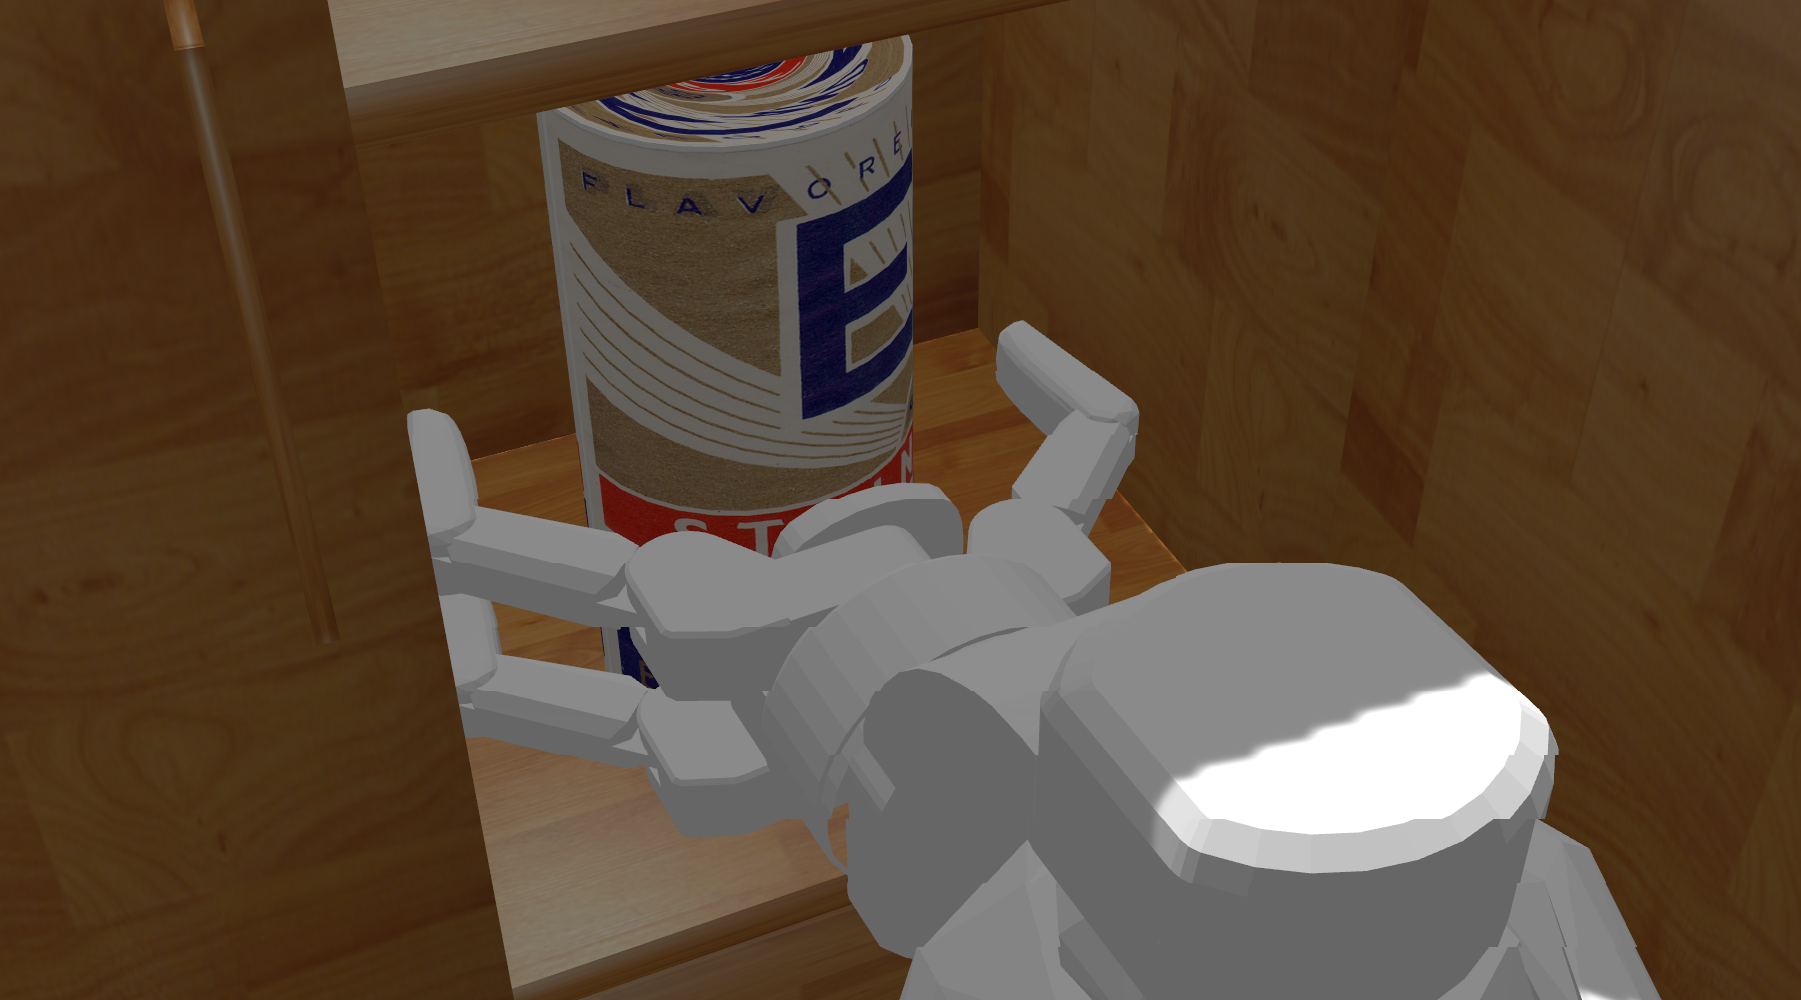
\includegraphics[scale=0.25]{images/testpuszka/chwyt.png}
        \caption{Przygotowanie chwytu}
    \end{figure}
\end{frame}

\addtocounter{framenumber}{-1}
\begin{frame}
	\frametitle{Wyciąganie puszki}
	\begin{figure}[b]
        \label{sim_map}
        \centering
        \def\svgwidth{\columnwidth}
        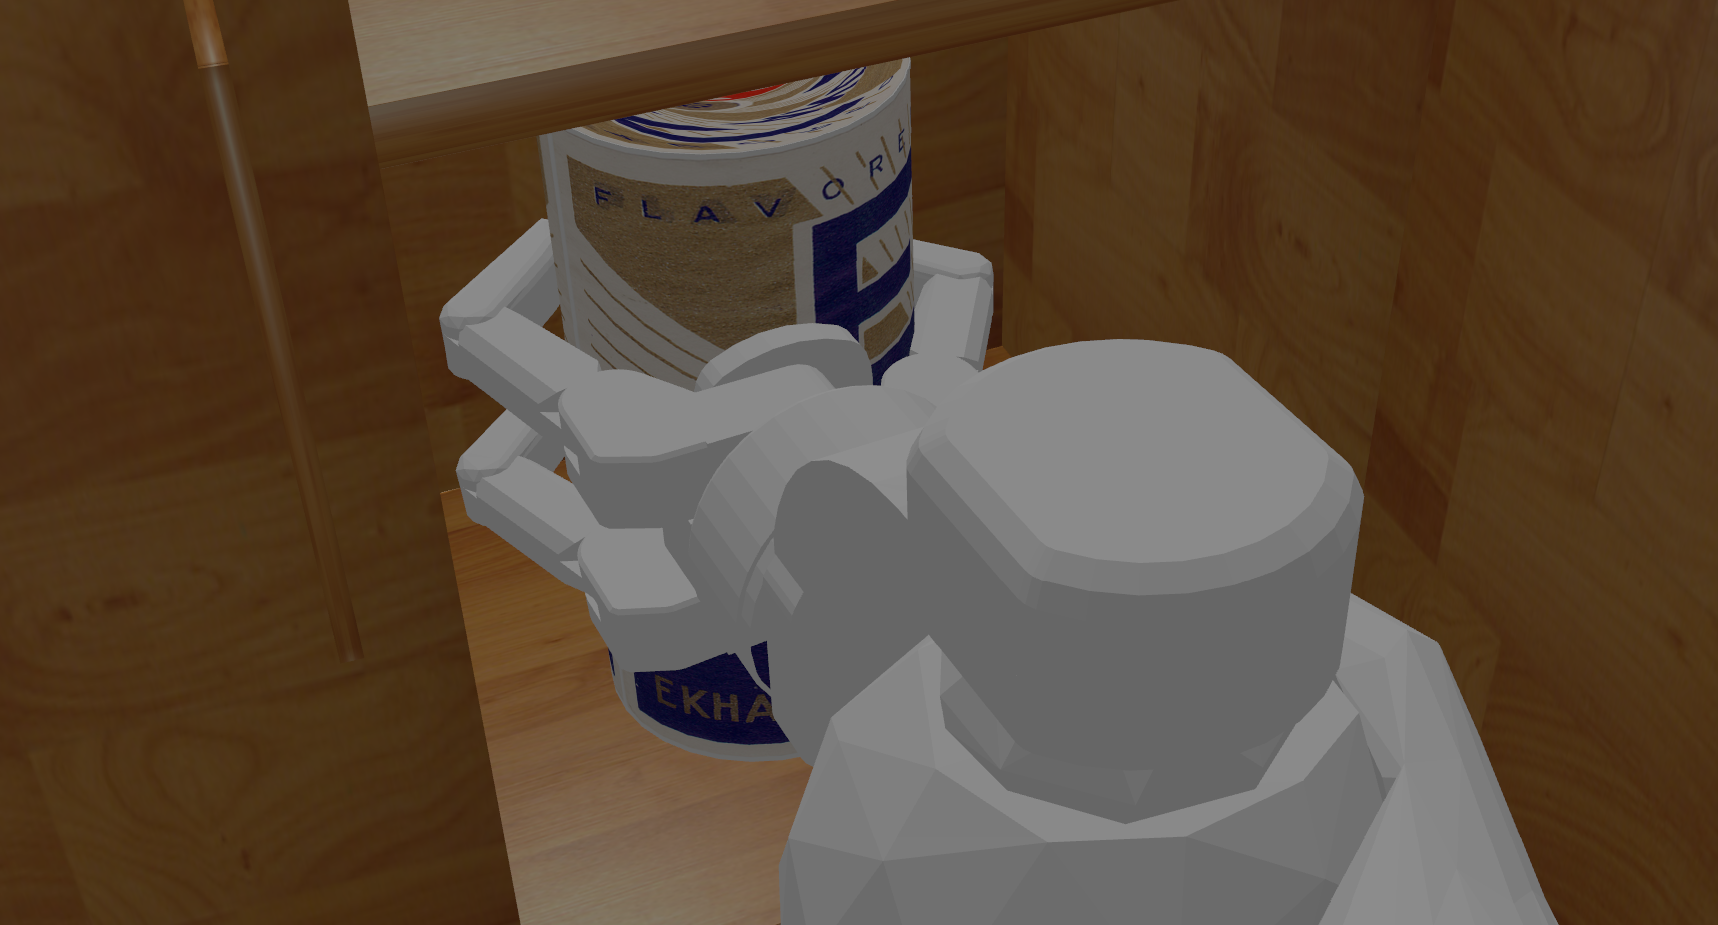
\includegraphics[scale=0.25]{images/testpuszka/chwyt_zacisniety.png}
        \caption{Realizacja chwytu}
    \end{figure}
\end{frame}

\addtocounter{framenumber}{-1}
\begin{frame}
	\frametitle{Wyciąganie puszki}
	\begin{figure}[b]
        \label{sim_map}
        \centering
        \def\svgwidth{\columnwidth}
        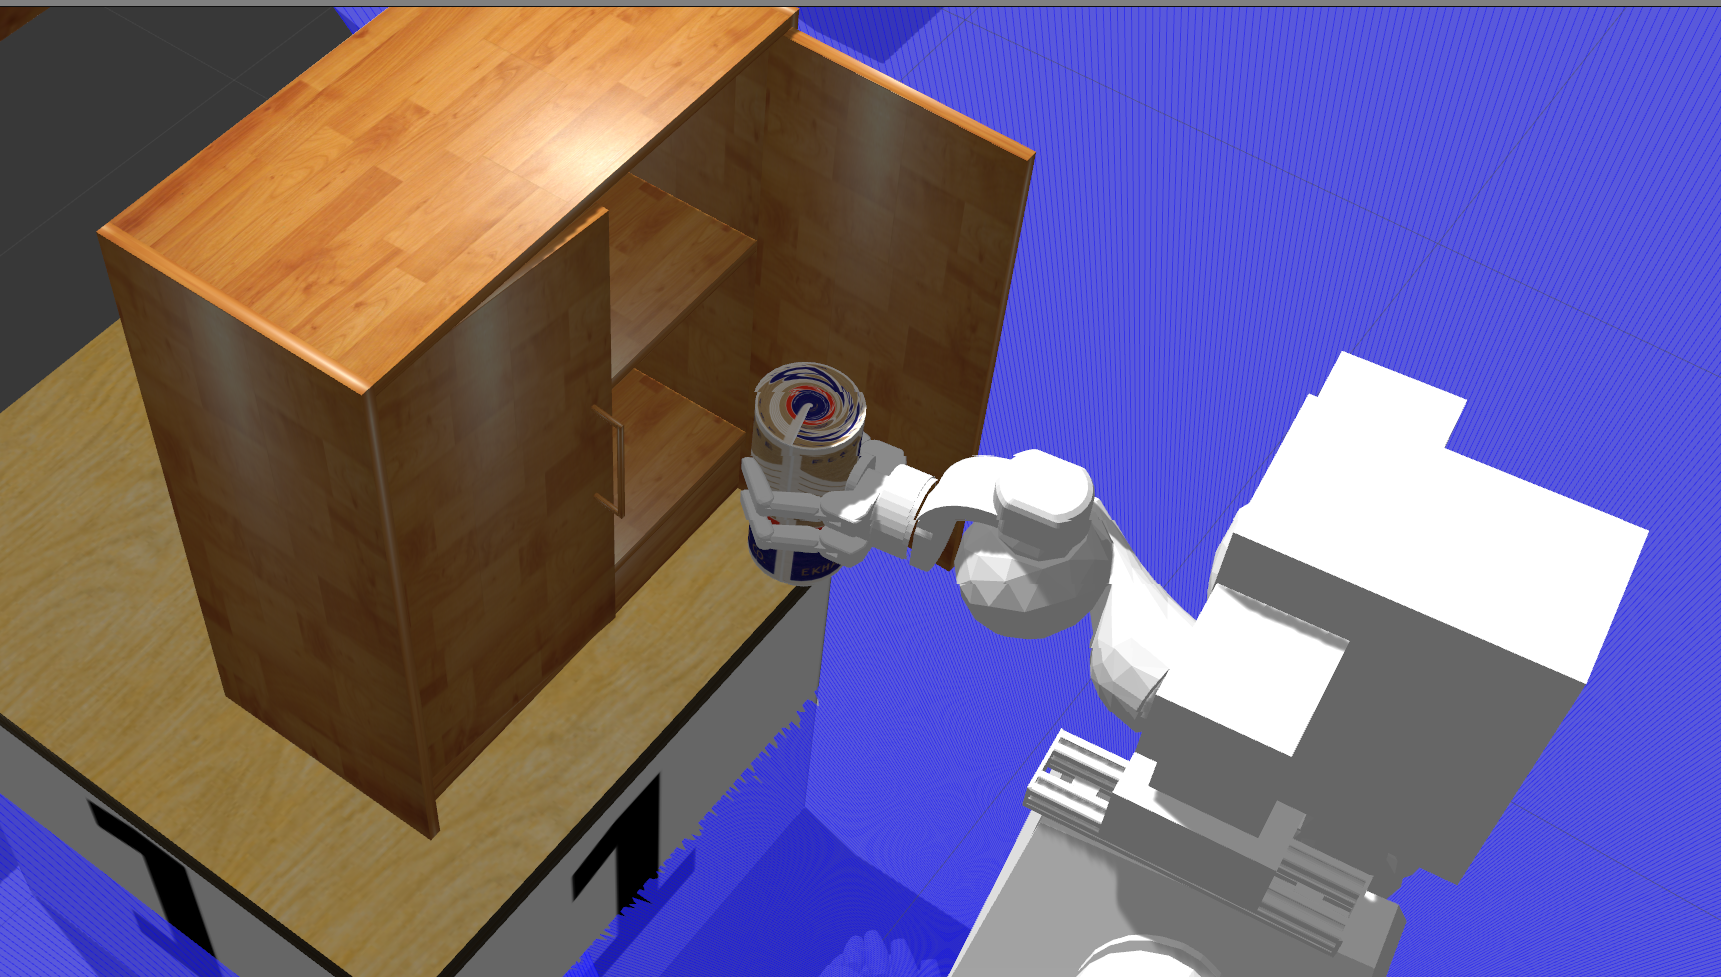
\includegraphics[scale=0.25]{images/testpuszka/wyciagniecie_puszki.png}
        \caption{Wyciąganie obiektu z szafki}
    \end{figure}
\end{frame}

\begin{frame}
	\frametitle{Odkładanie puszki}
	\begin{figure}[b]
        \label{sim_map}
        \centering
        \def\svgwidth{\columnwidth}
        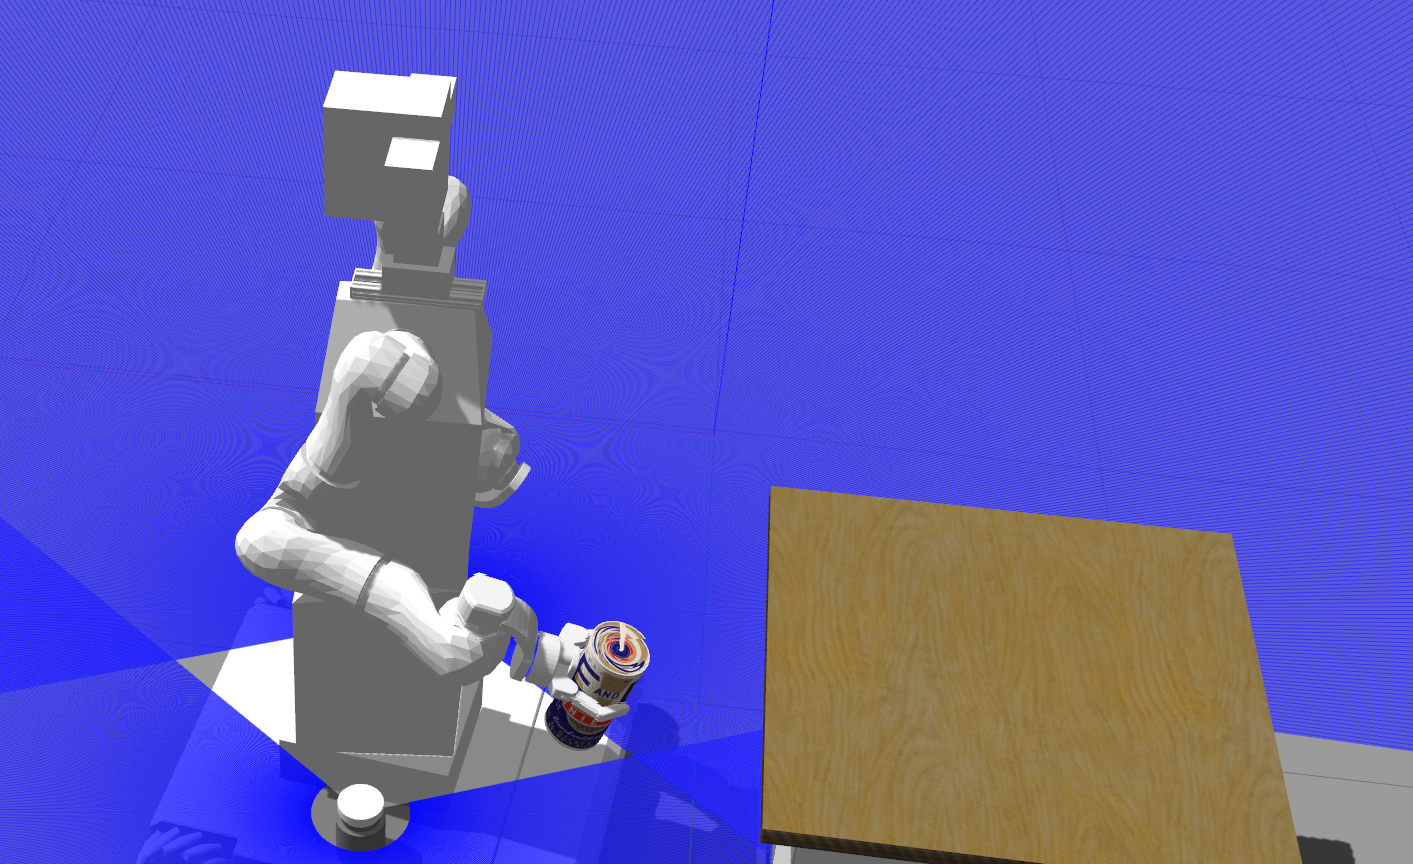
\includegraphics[scale=0.3]{images/testpuszka/dojazd_do_celu.png}
        \caption{Dojazd do stołu}
    \end{figure}
\end{frame}

\addtocounter{framenumber}{-1}
\begin{frame}
	\frametitle{Odkładanie puszki}
	\begin{figure}[b]
        \label{sim_map}
        \centering
        \def\svgwidth{\columnwidth}
        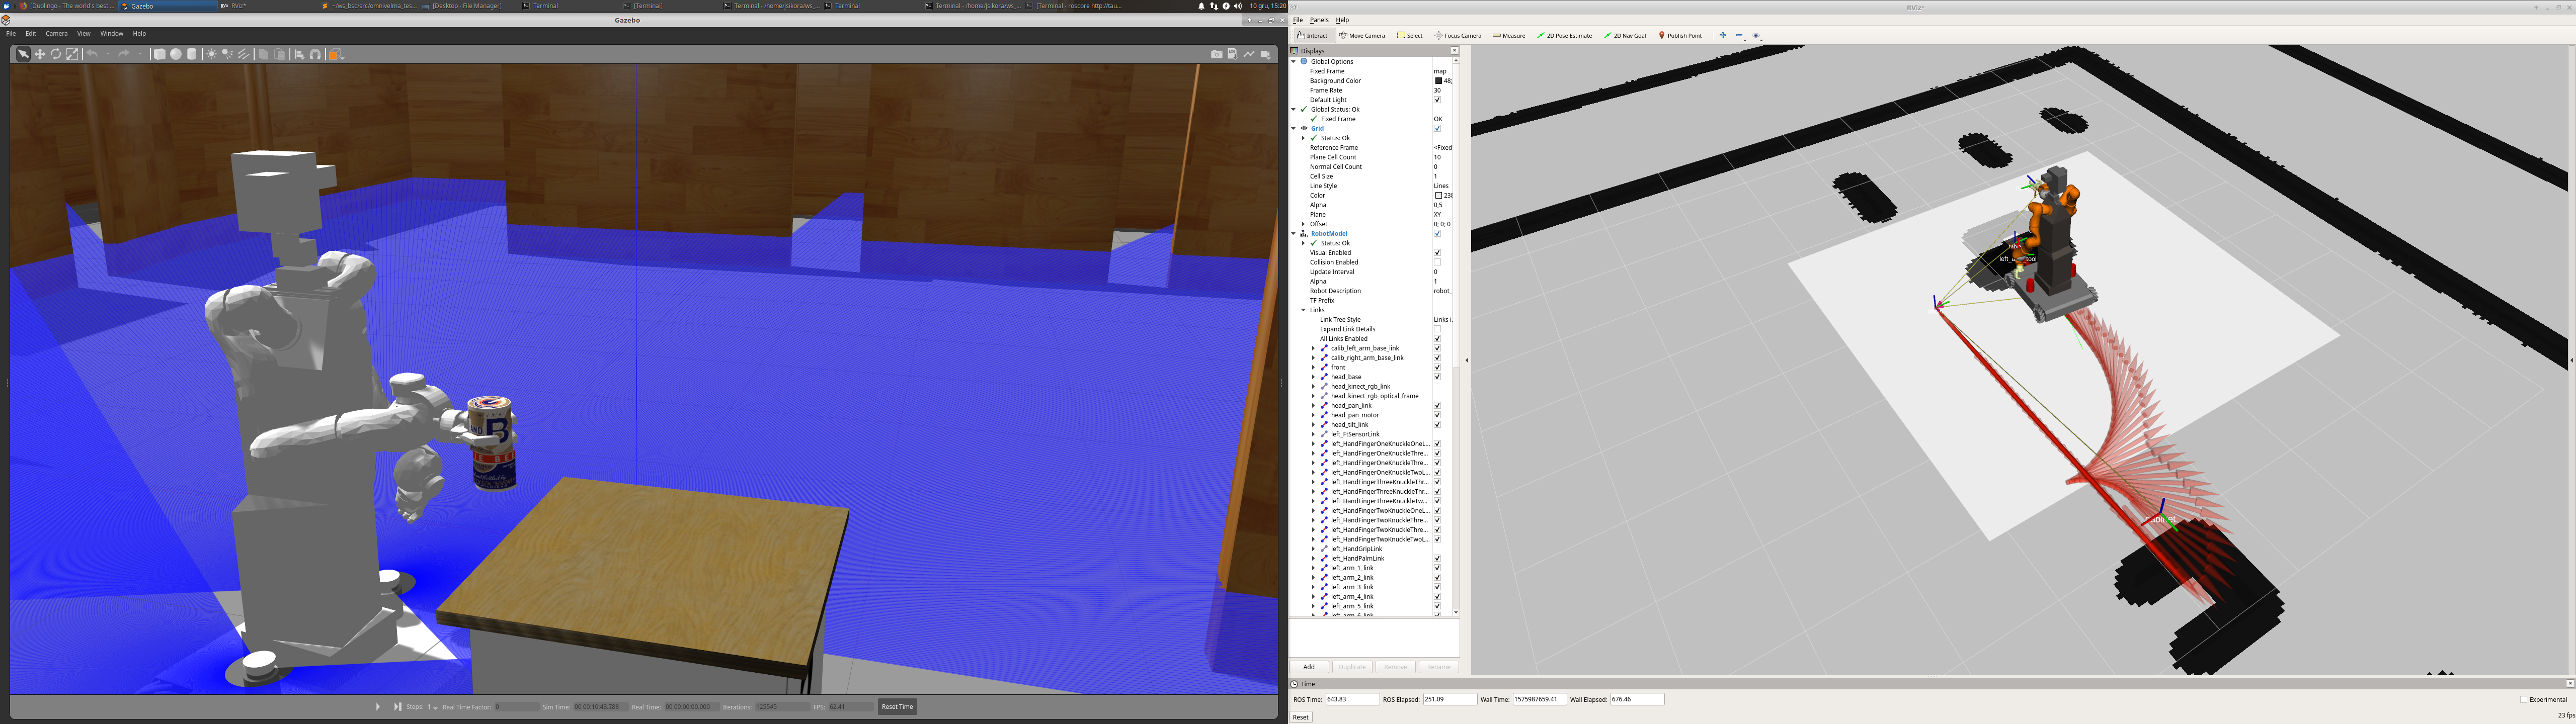
\includegraphics[scale=0.25]{images/testpuszka/odkladanie_puszki_start.png}
        \caption{Przeniesienie obiektu nad stół}
    \end{figure}
\end{frame}

\addtocounter{framenumber}{-1}
\begin{frame}
	\frametitle{Odkładanie puszki}
	\begin{figure}[b]
        \label{sim_map}
        \centering
        \def\svgwidth{\columnwidth}
        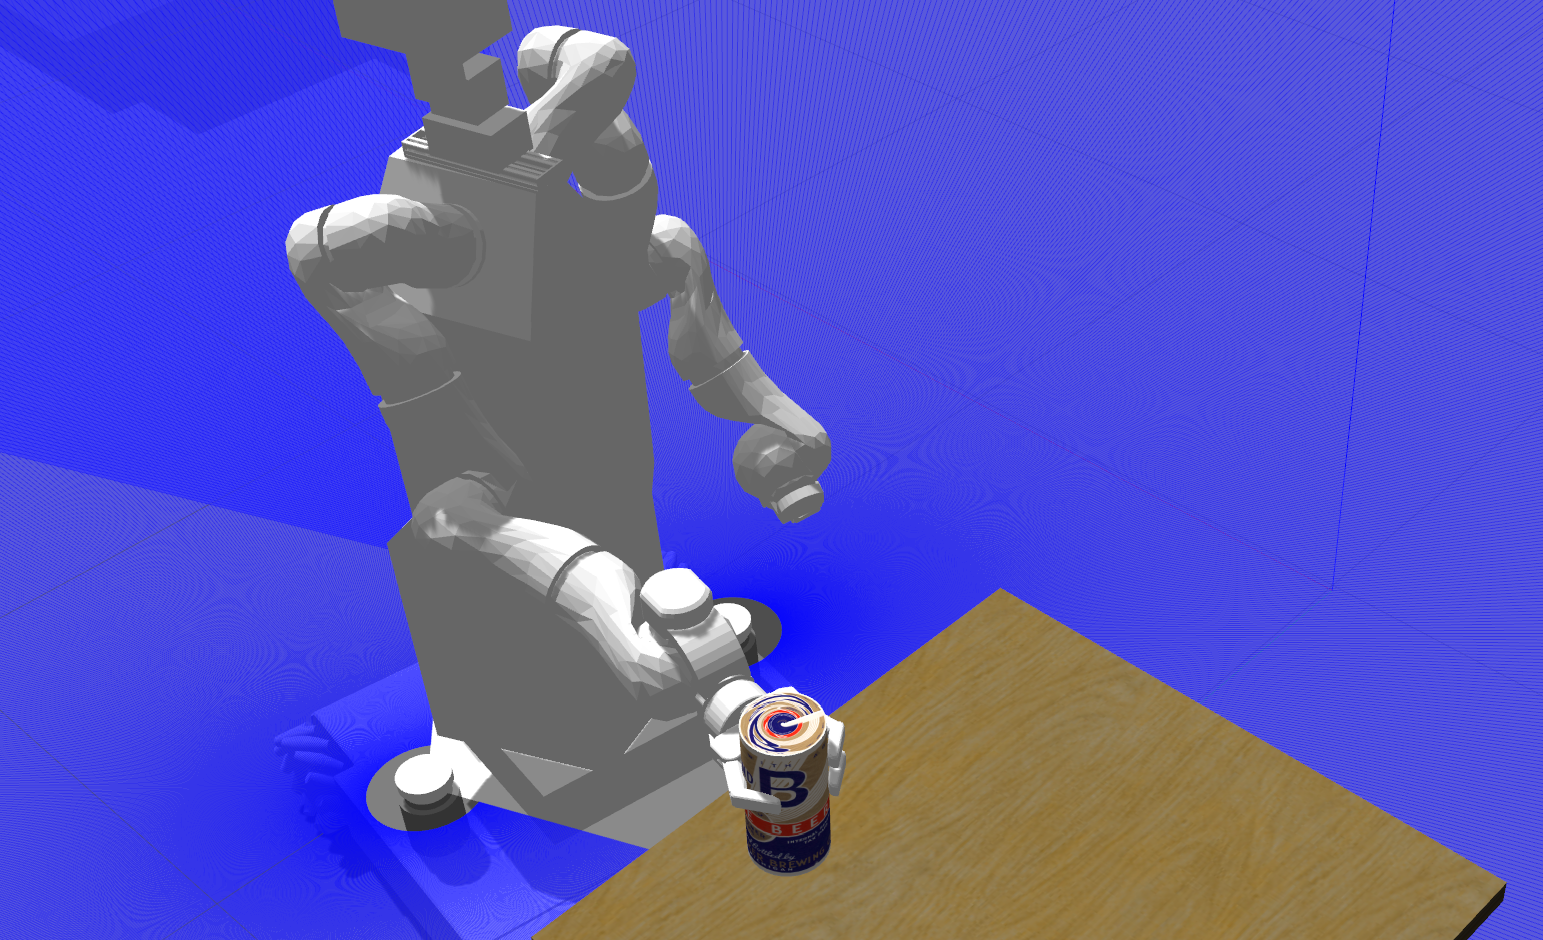
\includegraphics[scale=0.27]{images/testpuszka/odkladanie_puszki_cont.png}
        \caption{Odkładanie obiektu na stół}
    \end{figure}
\end{frame}

\addtocounter{framenumber}{-1}
\begin{frame}
	\frametitle{Odkładanie puszki}
	\begin{figure}[b]
        \label{sim_map}
        \centering
        \def\svgwidth{\columnwidth}
        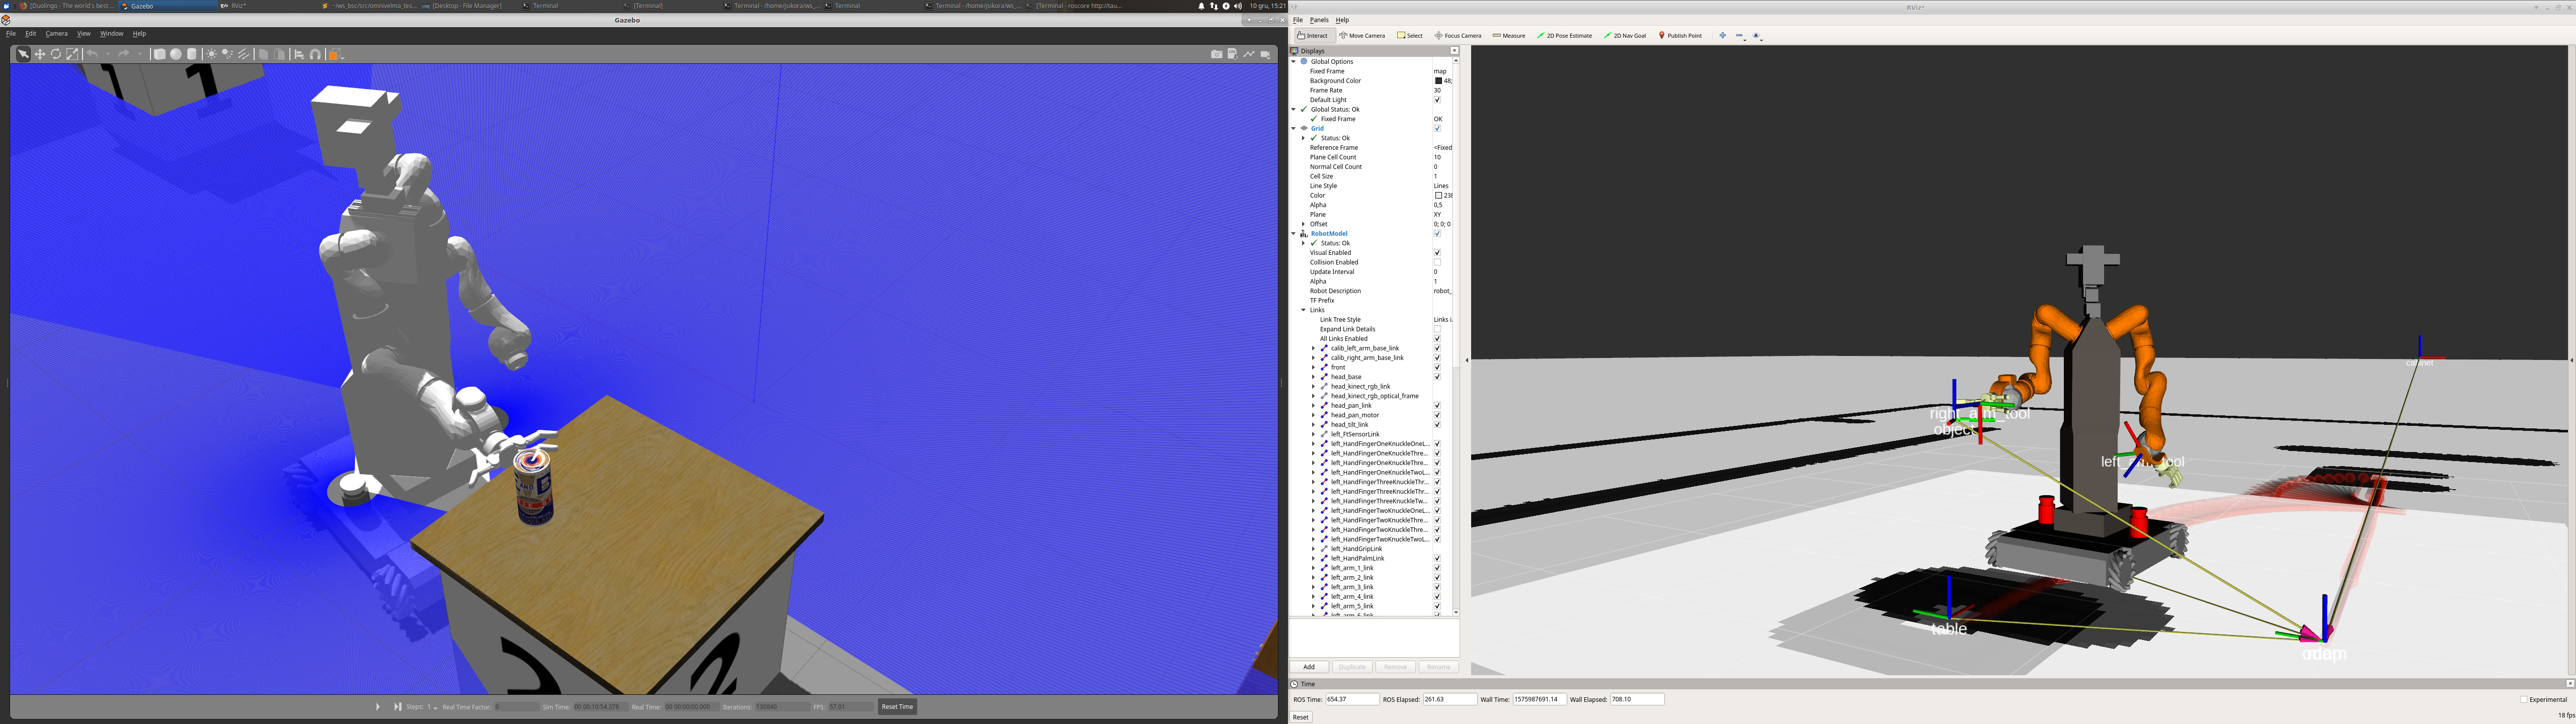
\includegraphics[scale=0.27]{images/testpuszka/puszka_na_stole.png}
        \caption{Zwolnienie chwytu}
    \end{figure}
\end{frame}

\addtocounter{framenumber}{-1}
\begin{frame}
	\frametitle{Odkładanie puszki}
	\begin{figure}[b]
        \label{sim_map}
        \centering
        \def\svgwidth{\columnwidth}
        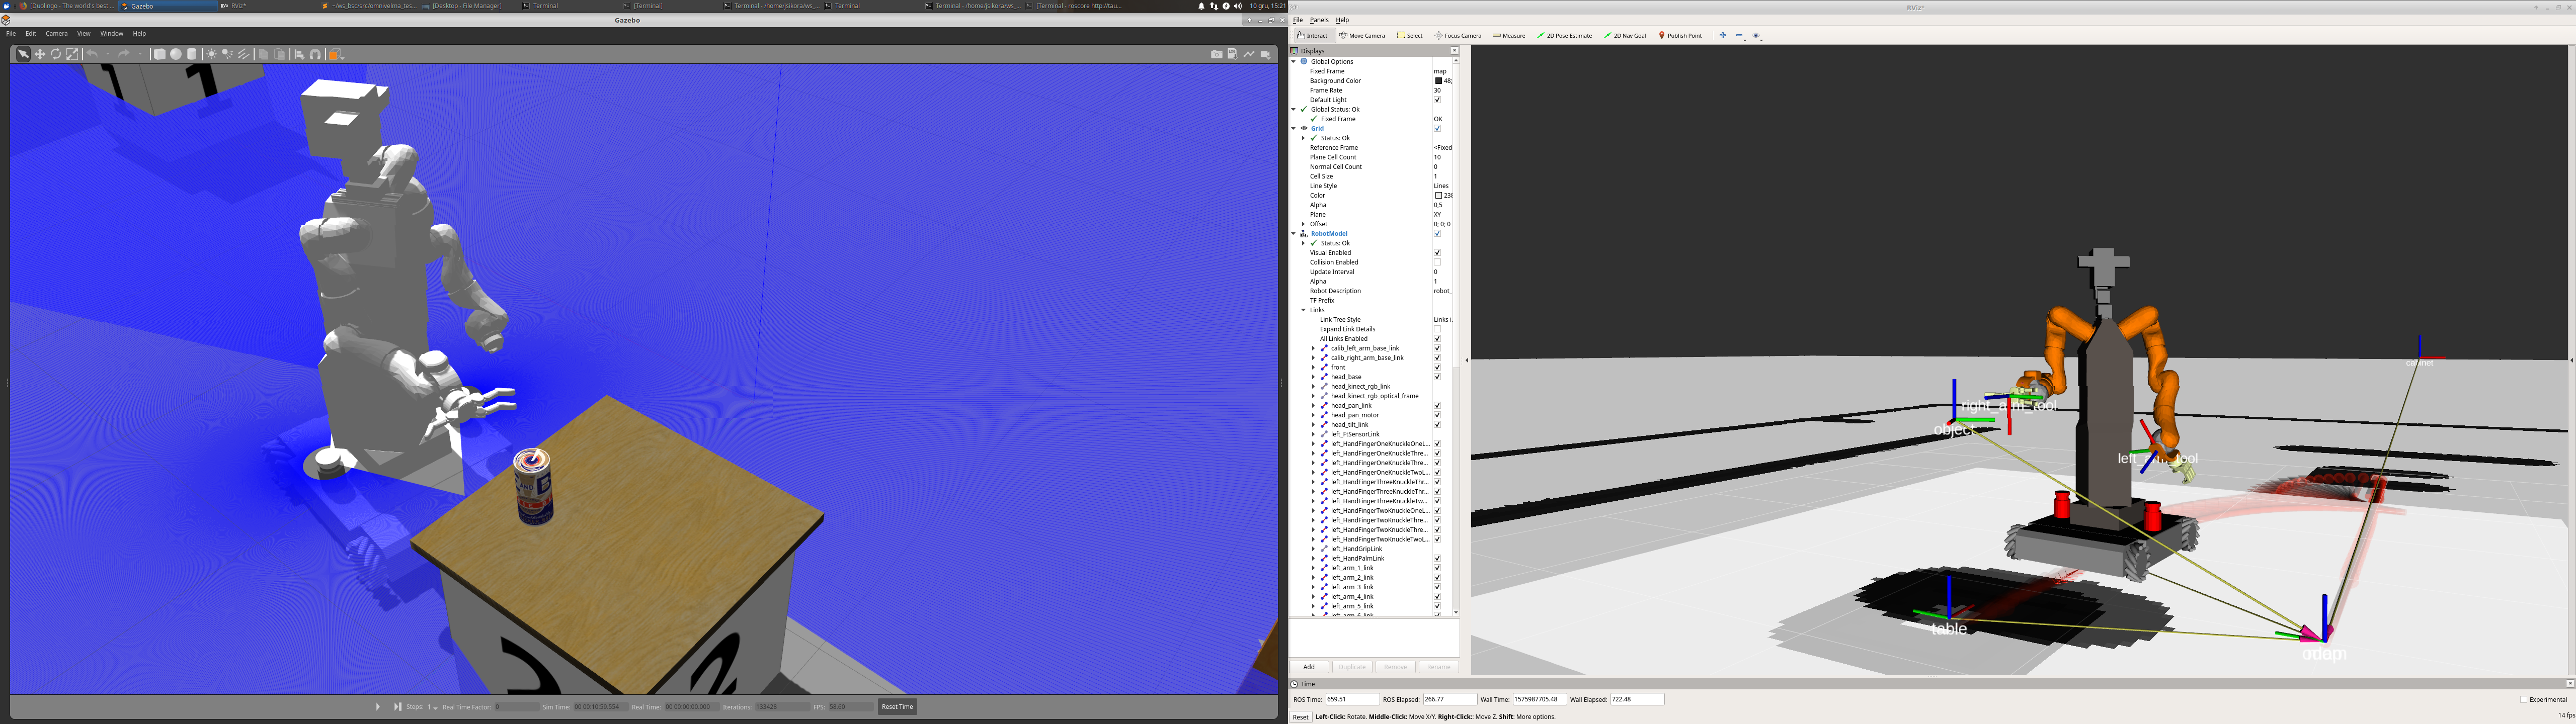
\includegraphics[scale=0.27]{images/testpuszka/odjazd_od_stolu.png}
        \caption{Cofnięcie chwytaka i powrót do pozycji początkowej}
    \end{figure}
\end{frame}


%%%%%%%%%%%%%%%%%%%%%%%%%%%%%%%%%%%%%%%%%%%%%
%% 			wykresy predkosci			   %%
%%%%%%%%%%%%%%%%%%%%%%%%%%%%%%%%%%%%%%%%%%%%%

\begin{frame}
\frametitle{Testowa trajektoria prędkości zadanej}
	\begin{figure}[t]
	    \centering
		 \begin{tikzpicture}
			\begin{axis}[
			width=0.95\textwidth,
			height=0.75\textheight,
			grid=major,
			xmin=0, xmax=50, ymin=-0.3, ymax=0.5,
			xlabel={$t$},
			ylabel={$v(t) / \omega(t)$},
			xtick={0, 10, 20, 30, 40, 50},
			legend pos=north west,
			legend style={nodes={scale=0.6, transform shape}, font={\large}},
			legend image post style={mark=-}],
			y tick label style={/pgf/number format/1000 sep=},
			]
				\addplot[blue, semithick] file{ ./data/controllers/cmd_vel_linear_x.csv };
			    \addplot[red, semithick] file{ ./data/controllers/cmd_vel_linear_y.csv };
			    \addplot[green, semithick] file{ ./data/controllers/cmd_vel_angular_z.csv };
			    \addlegendentry{$v_{x}(t)$},
			    \addlegendentry{$v_{y}(t)$},
			    \addlegendentry{$\omega(t)$},
			    \addlegendimage{no markers, blue}
			    \addlegendimage{no markers, red}
				\addlegendimage{no markers, green}
			    \end{axis}
		    \end{tikzpicture}
		\caption{Testowa trajektoria prędkości zadanej}
	\end{figure}
\end{frame}


\begin{frame}
\frametitle{Badania regulatorów prędkości zadanej}
	\begin{figure}[t]
	    \centering
		 \begin{tikzpicture}
			\begin{axis}[
			width=0.95\textwidth,
			height=0.75\textheight,
			grid=major,
			xmin=0, xmax=50, ymin=-0.2, ymax=0.3,
			xlabel={$t$},
			ylabel={$v(t)$},
			xtick={0, 10, 20, 30, 40, 50},
			legend pos=north west,
			legend style={nodes={scale=0.6, transform shape}, font={\large}},
			legend image post style={mark=-}],
			y tick label style={/pgf/number format/1000 sep=},
			]
				\addplot[blue, semithick] file{ ./data/controllers/odom_linear_x.csv };
			    \addplot[red, semithick] file{ ./data/controllers/cmd_vel_linear_x.csv };
			    \addlegendentry{$v^{\mathrm{zad}}_{x}(t)$},
			    \addlegendentry{$v_{x}(t)$},
			    \addlegendimage{no markers, red}
				\addlegendimage{no markers, blue}
			    \end{axis}
		    \end{tikzpicture}
		\caption{Porównanie przebiegów prędkości liniowej w osi x}
	\end{figure}
\end{frame}

\addtocounter{framenumber}{-1}
\begin{frame}
\frametitle{Badania regulatorów prędkości zadanej}
	\begin{figure}[t]
	    \centering
		 \begin{tikzpicture}
			\begin{axis}[
			width=0.95\textwidth,
			height=0.75\textheight,
			grid=major,
			xmin=0, xmax=50, ymin=-0.2, ymax=0.3,
			xlabel={$t$},
			ylabel={$v(t)$},
			xtick={0, 10, 20, 30, 40, 50},
			legend pos=north west,
			legend style={nodes={scale=0.6, transform shape}, font={\large}},
			legend image post style={mark=-}],
			y tick label style={/pgf/number format/1000 sep=},
			]
				\addplot[blue, semithick] file{ ./data/controllers/odom_linear_y.csv };
			    \addplot[red, semithick] file{ ./data/controllers/cmd_vel_linear_y.csv };
			    \addlegendentry{$v^{\mathrm{zad}}_{y}(t)$},
			    \addlegendentry{$v_{y}(t)$},
			    \addlegendimage{no markers, red}
				\addlegendimage{no markers, blue}
			    \end{axis}
		    \end{tikzpicture}
		\caption{Porównanie przebiegów prędkości liniowej w osi y}
	\end{figure}
\end{frame}

\addtocounter{framenumber}{-1}
\begin{frame}
\frametitle{Badania regulatorów prędkości zadanej}
	\begin{figure}[t]
	    \centering
		 \begin{tikzpicture}
			\begin{axis}[
			width=0.95\textwidth,
			height=0.75\textheight,
			grid=major,
			xmin=0, xmax=50, ymin=-0.3, ymax=0.6,
			xlabel={$t$},
			ylabel={$\omega(t)$},
			xtick={0, 10, 20, 30, 40, 50},
			legend pos=north west,
			legend style={nodes={scale=0.6, transform shape}, font={\large}},
			legend image post style={mark=-}],
			y tick label style={/pgf/number format/1000 sep=},
			]
				\addplot[blue, semithick] file{ ./data/controllers/odom_angular_z.csv };
			    \addplot[red, semithick] file{ ./data/controllers/cmd_vel_angular_z.csv };
			    \addlegendentry{$\omega^{\mathrm{zad}}(t)$},
			    \addlegendentry{$\omega(t)$},
			    \addlegendimage{no markers, red}
				\addlegendimage{no markers, blue}
			    \end{axis}
		    \end{tikzpicture}
		\caption{Porównanie przebiegów prędkości kątowej}
	\end{figure}
\end{frame}


%%%%%%%%%%%%%%%%%%%%%%%%%%%%%%%%%%%%%%%%%%%%%
%% 			wykresy odometrii			   %%
%%%%%%%%%%%%%%%%%%%%%%%%%%%%%%%%%%%%%%%%%%%%%

\begin{frame}
\frametitle{Badania regulatorów pozycji wzdłuż osi X}
	\begin{figure}[t]
	    \centering
		 \begin{tikzpicture}
			\begin{axis}[
			width=0.95\textwidth,
			height=0.75\textheight,
			grid=major,
			xmin=0, xmax=50, ymin=-0.03, ymax=0.03,
			xlabel={$t$},
			ylabel={$\Delta x(t)$},
			xtick={0, 10, 20, 30, 40, 50},
			ytick={-0.03, -0.015, 0.0, 0.015, 0.03},
			legend pos=north west,
			legend style={nodes={scale=0.6, transform shape}, font={\large}},
			legend image post style={mark=-}],
			y tick label style={/pgf/number format/1000 sep=},
			]
			    \addplot[red, semithick] file{ ./data/odometry/x_diffs.csv };
			    \addlegendentry{$\Delta x(t)$},
			    \addlegendimage{no markers, red}
			    \end{axis}
		    \end{tikzpicture}
		\caption{Błąd odometrii w osi X w trakcie realizowania testowej trajektorii prędkości}
	\end{figure}
\end{frame}

\addtocounter{framenumber}{-1}
\begin{frame}
\frametitle{Badania regulatorów pozycji wzdłuż osi Y}
	\begin{figure}[t]
	    \centering
		 \begin{tikzpicture}
			\begin{axis}[
			width=0.95\textwidth,
			height=0.75\textheight,
			grid=major,
			xmin=0, xmax=50, ymin=-0.03, ymax=0.03,
			xlabel={$t$},
			ylabel={$\Delta y(t)$},
			xtick={0, 10, 20, 30, 40, 50},
			ytick={-0.03, -0.015, 0.0, 0.015, 0.03},
			legend pos=north west,
			legend style={nodes={scale=0.6, transform shape}, font={\large}},
			legend image post style={mark=-}],
			y tick label style={/pgf/number format/1000 sep=},
			]
			    \addplot[red, semithick] file{ ./data/odometry/y_diffs.csv };
			    \addlegendentry{$\Delta y(t)$},
			    \addlegendimage{no markers, red}
			    \end{axis}
		    \end{tikzpicture}
		\caption{Błąd odometrii w osi Y w trakcie realizowania testowej trajektorii prędkości}
	\end{figure}
\end{frame}

\addtocounter{framenumber}{-1}
\begin{frame}
\frametitle{Badanie odometrii kąta $\gamma$}
	\begin{figure}[t]
	    \centering
		 \begin{tikzpicture}
			\begin{axis}[
			width=0.95\textwidth,
			height=0.75\textheight,
			grid=major,
			xmin=0, xmax=50, ymin=-0.05, ymax=0.05,
			xlabel={$t$},
			ylabel={$\Delta\gamma(t)$},
			xtick={0, 10, 20, 30, 40, 50},
			ytick={-0.05, -0.025, 0.0, 0.025, 0.05},
			legend pos=north west,
			legend style={nodes={scale=0.6, transform shape}, font={\large}},
			legend image post style={mark=-}],
			y tick label style={/pgf/number format/1000 sep=},
			]
			    \addplot[red, semithick] file{ ./data/odometry/yaw_diffs.csv };
			    \addlegendentry{$\Delta\gamma(t)$},
			    \addlegendimage{no markers, red}
			    \end{axis}
		    \end{tikzpicture}
		\caption{Błąd odometrii kąta $\gamma$ w trakcie realizowania testowej trajektorii prędkości}
	\end{figure}
\end{frame}

\begin{frame}
	\frametitle{Test stu obrotów}
	\begin{block}{Test stu obrotów}
		W ramach ostatniego testu, robot miał wykonać 100 obrotów wokół własnej osi, wykorzystując
		do tego bazę mobilną.
	\end{block}
	\begin{table}[]
		\begin{tabular}{c|c|c|c}
			   & x $[m]$       & y $[m]$     & $\gamma$ $[rad]$  \\ \hline
		Gazebo & $\num{-0.0188}$ & $\num{-0.0176}$ & $\num{-0.4894}$  \\ \hline
		Odom   & $\num{0.2188}$ & $\num{-0.1611}$ & $\num{0.5950}$ \\ \hline \hline
		Różnica & $\num{-0.2127}$ & $\num{0.1709}$  & $\num{-1.0845}$ 
		\end{tabular}
	\end{table}
\end{frame}